%!TEX TS-program = xelatex

\documentclass[xetex,mathserif,serif,t]{beamer}
% Если хотим соотношение сторон 16:9
% \documentclass[aspectratio=169,xetex,mathserif,serif,t]{beamer}

%%% Преамбула
\usetheme{MasterThesis} % Тема

%%% Работа с русским языком
\usepackage{fontspec,xunicode,xltxtra}

\defaultfontfeatures{Ligatures=TeX} % Для преобразования -- и ---
\setmainfont{PT Sans}
\setmonofont{PT Mono}

%%% Beamer по-русски
\newtheorem{rtheorem}{Теорема}
\newtheorem{rproof}{Доказательство}
\newtheorem{rexample}{Пример}

%%% Дополнительная работа с математикой
\usepackage{amsmath,amsfonts,amssymb,amsthm,mathtools} % AMS
\usepackage{icomma} % "Умная" запятая: $0,2$ --- число, $0, 2$ --- перечисление

%%% Свои команды
\DeclareMathOperator{\sgn}{\mathop{sgn}}

%%% Перенос знаков в формулах (по Львовскому)
\newcommand*{\hm}[1]{#1\nobreak\discretionary{}
{\hbox{$\mathsurround=0pt #1$}}{}}

%%% Работа с картинками
\usepackage{graphicx}    % Для вставки рисунков
\graphicspath{{../images/}} % Каталоги с картинками
\setlength\fboxsep{3pt}  % Отступ рамки \fbox{} от рисунка
\setlength\fboxrule{1pt} % Толщина линий рамки \fbox{}
\usepackage{wrapfig}     % Обтекание рисунков текстом

%%% Работа с таблицами
\usepackage{array,tabularx,tabulary,booktabs} % Дополнительная работа с таблицами
\usepackage{longtable}  % Длинные таблицы
\usepackage{multirow}   % Слияние строк в таблице

%%% Другие пакеты
\usepackage{lastpage} % Узнать, сколько всего страниц в документе
\usepackage{soulutf8} % Модификаторы начертания
\usepackage{csquotes} % Еще инструменты для ссылок
\usepackage{multicol} % Несколько колонок
\usepackage{etoolbox} % Логические операторы

%%% Картинки
\usepackage{tikz,calc,ifthen,color}

\title{Решение прямой задачи бокового каротажного зондирования методами численного моделирования}
\subtitle{Выпускная квалификационная работа по программе бакалавриата на тему:}
\author{Докладчик:\\
ст.гр.~4Ф-3,~Кадыров~А.В. \\
\vspace{0.7\baselineskip}
Научный руководитель:\\
к.ф.-м.н.,~доцент,~Ремеев~И.С.}
\institute{Башкирский государственный университет \\
Кафедра геофизики}
\date{2020~г.}

\begin{document}
%%% Содержимое слайдов

% 1. Название, автор, руководитель.
% 2. Постановка задачи (актуальность)
% 3. способ (инструменты для) решения
% 4. результаты
% 5. анализ результатов
% 6. Заключение 

\frame[plain]{\titlepage} % Титульный слайд

%-------------------------------------------------------------------------------

\section{Постановка задачи}

\begin{frame}
\frametitle{\insertsection}

\begin{itemize}    
    \item палетки с любыми параметрами (без ограничений времени)
    \item оценка возможности решения обратной задачи БКЗ в реальном времени
\end{itemize}

\textbf{Математическая постановка:}
\begin{alignat}{2}
\nabla \cdot (\nabla u(\bm x) / \rho(\bm x)) &= f(\bm x),\qquad && \bm x \in \Omega, \label{eq:poisson}\\
u(\bm x) &= 0, && \bm x \in \partial \Omega. \label{eq:dirichet}
\end{alignat}

\textbf{Источниковый член}:
\begin{equation}
f(\bm x) = -I \delta(\bm x).
\end{equation}
\end{frame}

\begin{frame}
\frametitle{\insertsection}

\begin{minipage}[t]{0.47\linewidth}
    \textbf{Модель 1}
    \center{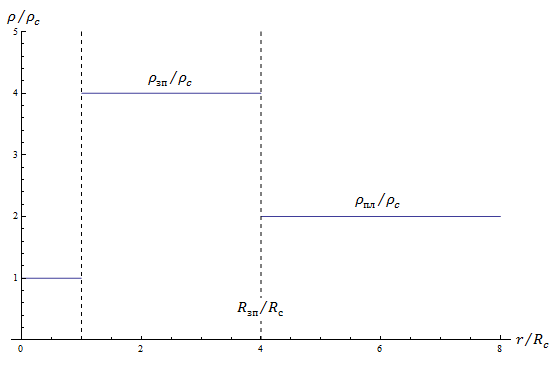
\includegraphics[width=1\linewidth]{rho_model_1.png}}
\end{minipage}
\hfill
\begin{minipage}[t]{0.47\linewidth}
    \textbf{Модель 2}
    \center{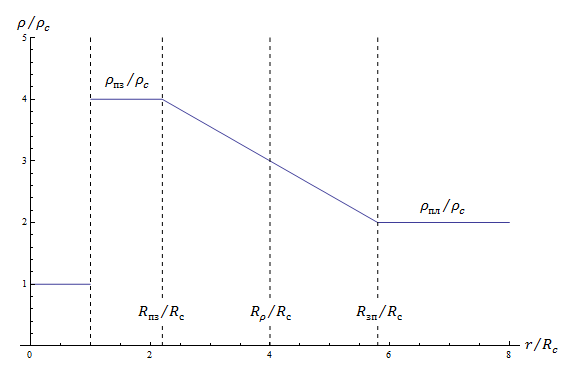
\includegraphics[width=1\linewidth]{rho_model_2.png}}
\end{minipage}
\end{frame}
%-------------------------------------------------------------------------------

\section{Способ решения}

\begin{frame}
\frametitle{\insertsection}

\textbf{Инструменты:}
\begin{itemize}
    \item Язык программирования Python
    \item Вычислительная платформа FEniCS
    \item Модуль triangle для триангуляции Делоне
    \item Компьютер: ОС Ubuntu 18.04 LTS, процессор Intel Pentium 4415U 2.30 ГГц
\end{itemize}
\end{frame}

%-------------------------------------------------------------------------------

\section{Результаты}

\begin{frame}
\frametitle{\insertsection}

\vspace{-0.5cm}
\begin{minipage}[t]{0.47\linewidth}
    \textbf{Модель 1}
    \center{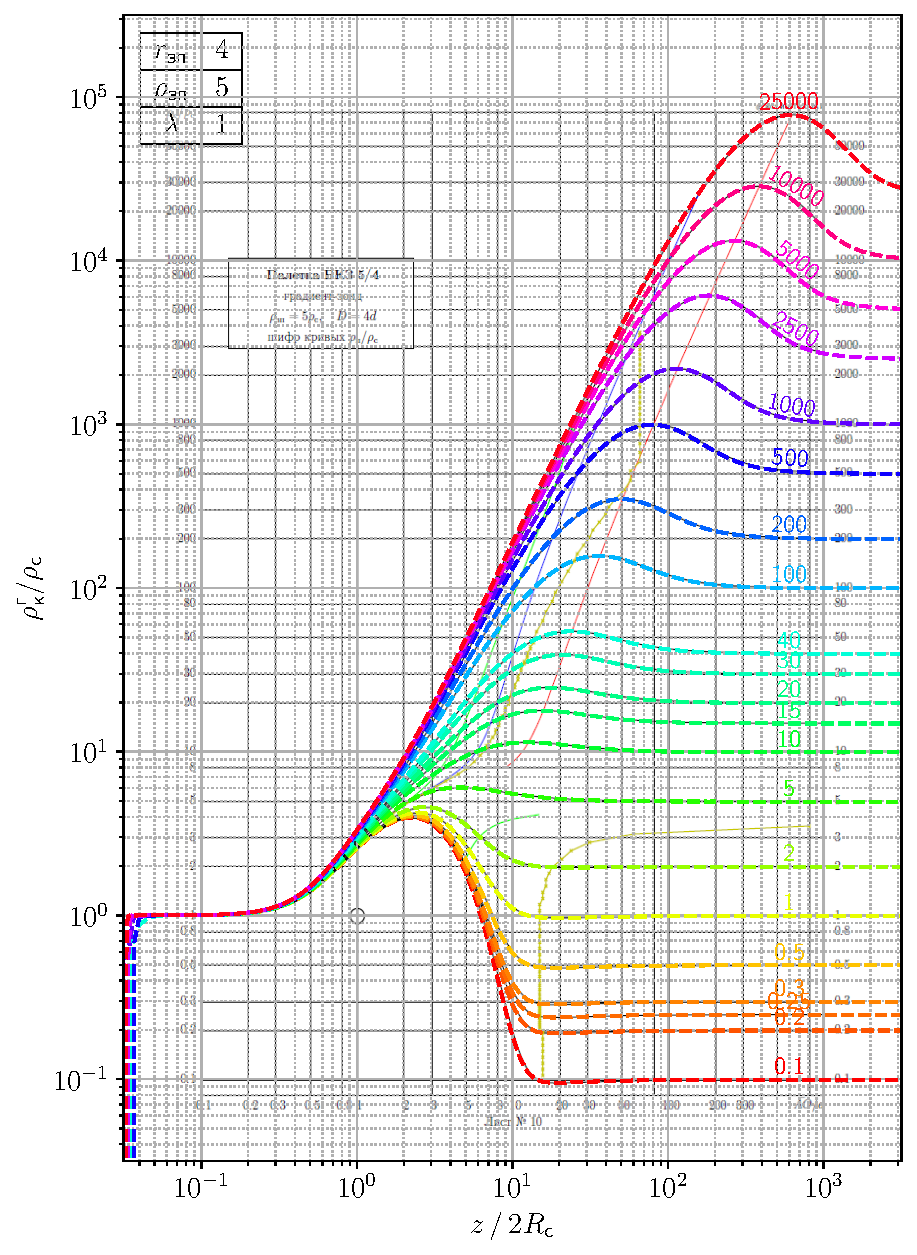
\includegraphics[width=1\linewidth]{plot_1_compare}}
\end{minipage}
\hfill
\begin{minipage}[t]{0.47\linewidth}
    \textbf{Модель 2}
    \center{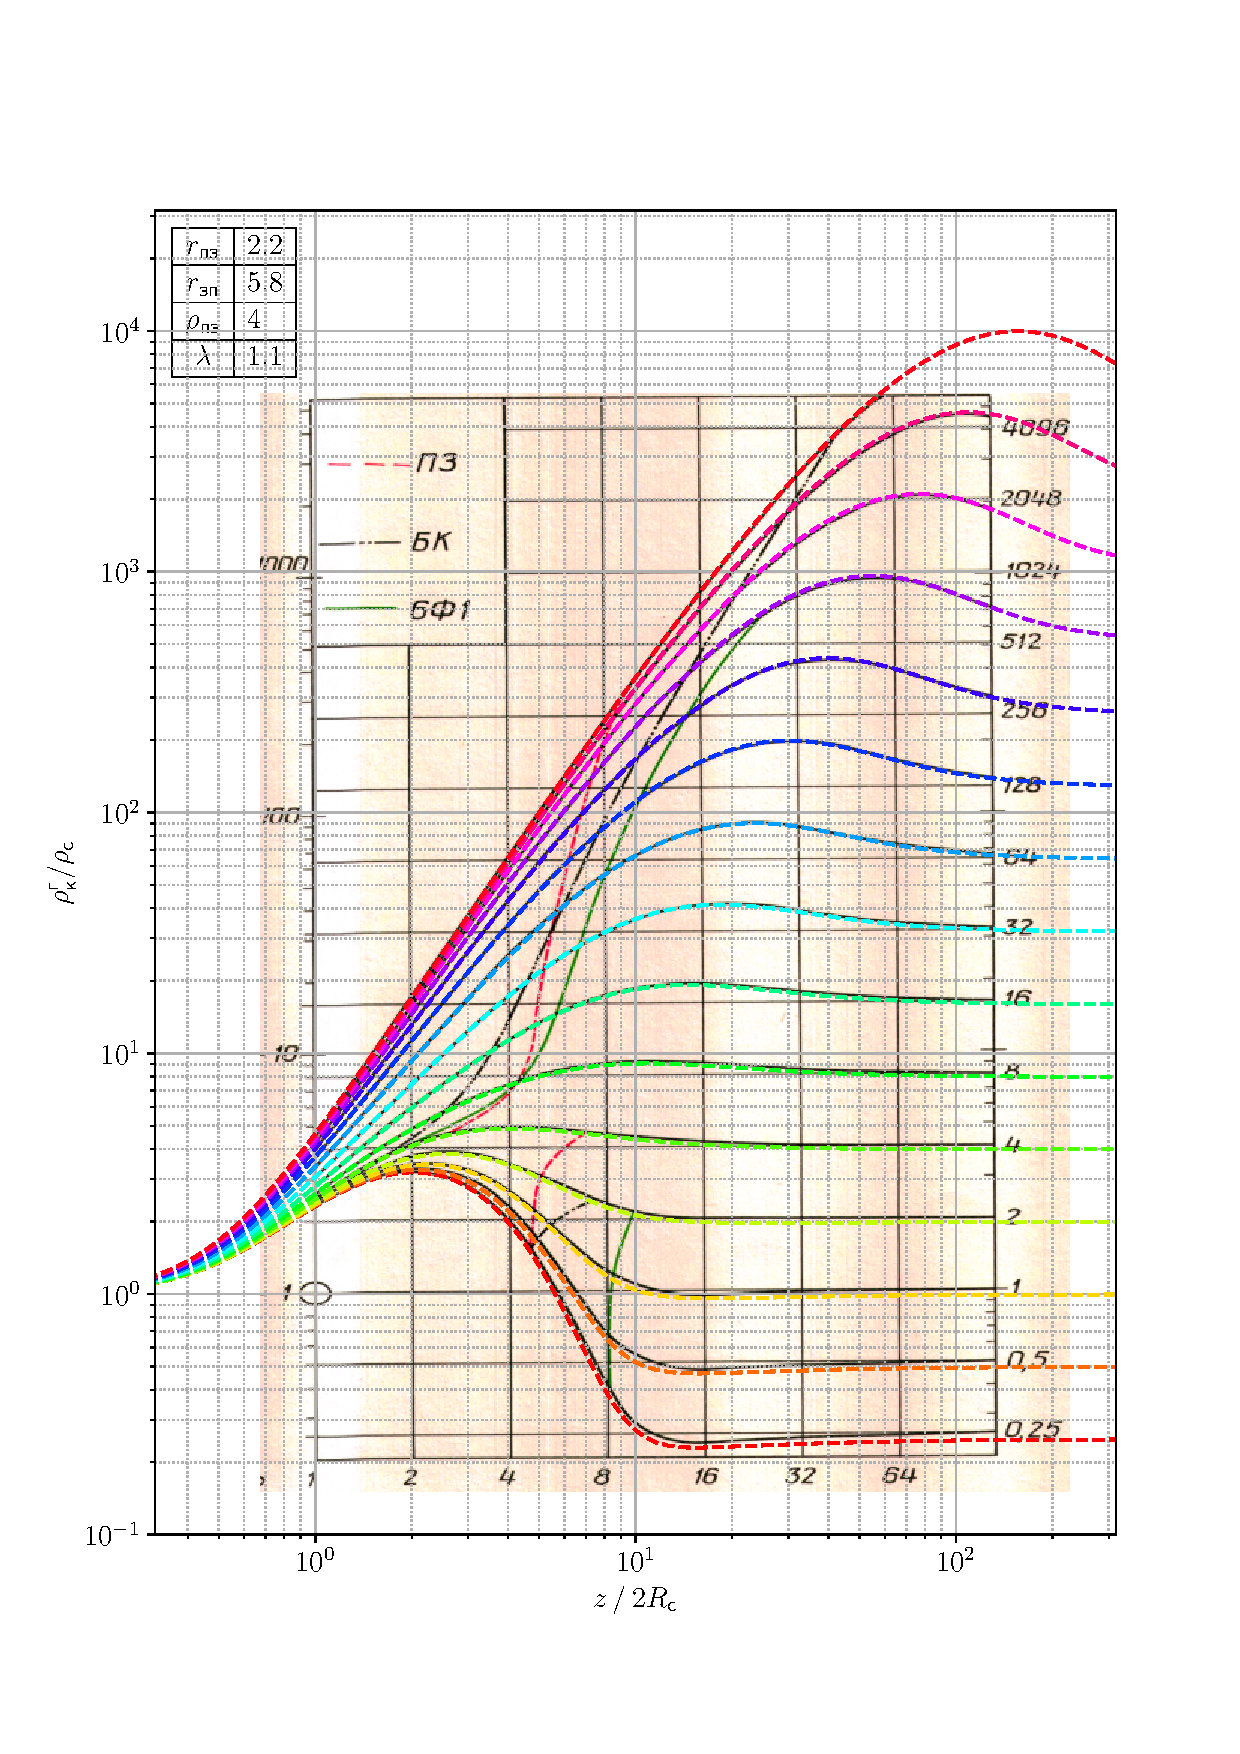
\includegraphics[width=1\linewidth]{plot_2_compare}}
\end{minipage}

\end{frame}

%-------------------------------------------------------------------------------

\section{Анализ результатов}

\begin{frame}
\frametitle{\insertsection}

\textbf{Модель 1:}
\begin{itemize}
    \item Время вычисления расчетной палетки 1 мин 32 с
\end{itemize}
\bigskip

\textbf{Модель 2:}
\begin{itemize}
    \item Время вычисления расчетной палетки 18.7 c
\end{itemize}
\bigskip

\textbf{Критерии точности решения}:
\begin{itemize}
    \item гладкость решения
    \item сравнение "на глаз" решения с известным
\end{itemize}
\end{frame}

%-------------------------------------------------------------------------------

\section{Заключение}

\begin{frame}
\frametitle{\insertsection}

\begin{itemize}
    \item Освоены пакеты программ для параллельных вычислений
    \item Проведены расчеты и сопоставление с известными результатами в литературе
    \item Показана применимость метода решения прямой задачи БКЗ
\end{itemize}
\end{frame}

%-------------------------------------------------------------------------------

\section{Конец}

\begin{frame}
\centering
\vfill
\textcolor{Blue}{\Large Спасибо за внимание!}
\vfill
\end{frame}
\end{document}
